% - template colors
\documentclass{beamer}

% SETUP
\usepackage{morris}
\definecolor{purple}{rgb}	{0.69, 0.38, 0.53}
\definecolor{orange}{rgb}	{0.84, 0.36, 0.05}
\definecolor{blue}{rgb}	{0.27, 0.52, 0.53}
\definecolor{green}{rgb}	{0.6, 0.59, 0.1}
\definecolor{red}{rgb}	{0.8, 0.14, 0.11}
\definecolor{yellow}{rgb}	{0.84, 0.6, 0.13}
\definecolor{aqua}{rgb}	{0.41, 0.62, 0.42}
\definecolor{extlinkcolor}{rgb}	{0.03, 0.4, 0.47}
\definecolor{intlinkcolor}{rgb}	{0.69, 0.23, 0.01}

\DeclareMathOperator{\elbo}{ELBO}
\DeclareMathOperator*{\erf}{erf}

\newcommand{\aprxpost}{{q_{\B{\φ}_k}(\s_k|\m)}}

% Following are some really short macros!
\newcommand\D{\ensuremath{\mathcal{D}}}
\newcommand\m{\ensuremath{\B{m}}}
\newcommand\s{\ensuremath{\B{s}}}
\newcommand\z{\ensuremath{\B{z}}}
\newcommand\x{\ensuremath{\B{x}}}

\newcommand{\decrvalue}[2]{\the\numexpr\value{#1}-#2\relax}


\definecolor{primary}{HTML}{524667}

\usetheme[numbering=fraction,block=fill]{metropolis}
\setbeamercolor{normal text}{fg=black, bg=white}

\setbeamercolor{palette primary}{%
    fg=white,
    bg=primary
}

\graphicspath{{graphics/}} % set of paths to search for images

\usepackage{tikz}
\usepackage{tikz-bayesnet}
\usetikzlibrary{
    3d,
    arrows,
    arrows.meta,
    backgrounds,
    bending,
    calc,
    chains,
    decorations.pathmorphing,
    decorations.pathreplacing,
    graphs,
    matrix,
    patterns,
    positioning,
    quotes,
    shapes.arrows,
    shapes.geometric,
    shapes.misc,
}
\tikzset{>=latex}
% \tikzset{every picture/.style={/utils/exec={\sffamily}}}

\usepackage{pgfplots}
\usepgfplotslibrary{
    groupplots,
    dateplot,
}
\pgfplotsset{compat=newest}
\usepackage[size=footnotesize]{subcaption}
\usepackage[font=footnotesize]{caption}

\usefonttheme{serif}
\usefonttheme{professionalfonts}
\usepackage{mathpazo}
\usepackage{euler}
\usepackage[export]{adjustbox}
\setbeamerfont{footnote}{size=\tiny}


\setbeamertemplate{title page}[default]

\usepackage[many]{tcolorbox}
% ---------------------------------------------------------------------------------------------------------------------------------------


% META DATA
\title{Problems using deep generative models for
probabilistic audio source separation}
\date{\today}
\author{}
\institute{\textsc{amsterdam machine learning lab\\university of amsterdam}}

\setbeamertemplate{title page}{
  \begin{minipage}[b][\paperheight]{\textwidth}
    \ifx\inserttitlegraphic\@empty\else\usebeamertemplate*{title graphic}\fi
    \vfill%
    \ifx\inserttitle\@empty\else\usebeamertemplate*{title}\fi
    \ifx\insertsubtitle\@empty\else\usebeamertemplate*{subtitle}\fi
    \usebeamertemplate*{title separator}
    % \ifx\beamer@shortauthor\@empty\else\usebeamertemplate*{author}\fi
    % \ifx\insertdate\@empty\else\usebeamertemplate*{date}\fi
    \ifx\insertinstitute\@empty\else\usebeamertemplate*{institute}\fi
    \vspace*{0.5cm}
    \begin{tikzpicture}[scale=1, every node/.style={scale=0.9}]
        \node[circle,draw,inner sep=0.5cm,fill overzoom image=frank] (frank) {};
        \node[right=3.7cm of frank,circle,draw,inner sep=0.5cm,fill overzoom image=ilse] (ilse) {};
        \node[below=0.2cm of frank,align=center] (franktext) {Maurice Frank\\@morris\_frank\_\\maurice.frank@posteo.de};
        \node[below=0.2cm of ilse,align=center] (ilsetext) {Maximilian Ilse\\@MaxIlse\\m.ilse@uva.nl};
        \node [anchor=west,fill=primary,text width=4cm,text=white,scale=0.8,rotate=-15] (note) at (0.2,1) {Searching for PhD in these topics!};
        \draw [-latex, ultra thick, primary] (note.south) to[out=-40, in=-20] (frank.east);
    \end{tikzpicture}
    \vfill
    \vspace*{1mm}
  \end{minipage}
}

\begin{document}
    \maketitle

    \begin{frame}{Cross-likelihood of the noiseless models}
        \begin{figure}
            \centering
            \adjustbox{minipage=0em,valign=t}{}%
        \put(20,60){\makebox[0pt][r]{FloWaveNet}}%
        \put(20,-40){\makebox[0pt][r]{WaveNet}}%
        \hspace{2em}
        \begin{subfigure}{0.29\textwidth}
            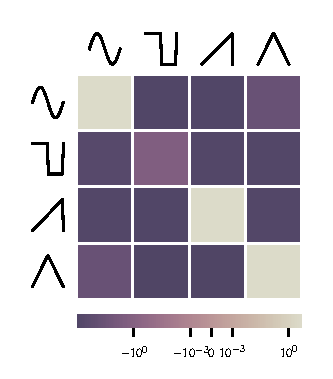
\includegraphics[width=\textwidth]{toy_noise_0/channels_hm}\\%
            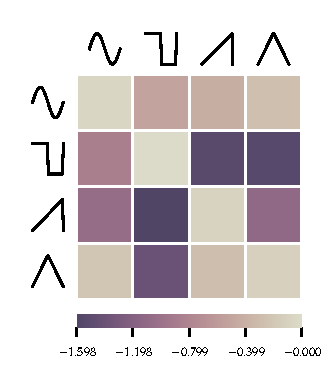
\includegraphics[width=\textwidth]{toy_noise_0/wn_channels_hm}%
            \caption{Toy dataset}%
        \end{subfigure}
        \begin{subfigure}{0.29\textwidth}
            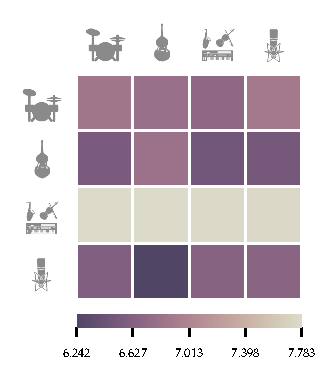
\includegraphics[width=\textwidth]{musdb_noiseless/channels_hm}\\%
            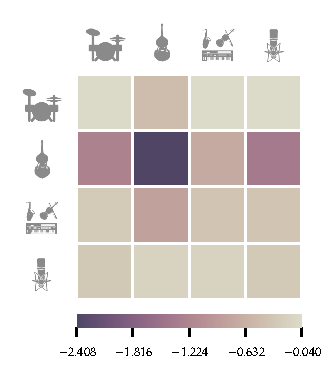
\includegraphics[width=\textwidth]{musdb_noiseless/wn_channels_hm}%
            \caption{\texttt{musdb18} dataset}%
        \end{subfigure}
        \end{figure}
    \end{frame}

    \begin{frame}{Fine-tune with noisy samples}
        \begin{figure}
            \centering
            \adjustbox{minipage=0em,valign=t}{}%
        \put(20,42){\makebox[0pt][r]{FloWaveNet}}%
        \put(20,-30){\makebox[0pt][r]{WaveNet}}%
        \hspace{1.4em}
        \foreach\level in {0, 01,027,129}{
            \begin{subfigure}{0.19\textwidth}
                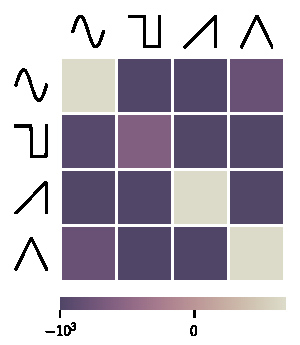
\includegraphics[width=\textwidth]{toy_noise_\level/channels_hm}\\%
                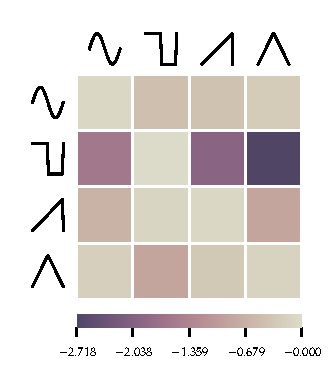
\includegraphics[width=\textwidth]{toy_noise_\level/wn_channels_hm}%
                \caption{\(\sigma = 0.\level\)}%
            \end{subfigure}
        }%
        \end{figure}
    \end{frame}

    \begin{frame}{Conclusion}
        \centering
        \begin{tikzpicture}
            \node[align=center] (pickone) {For your generative audio priors,\\ pick one:};
            \node[draw,circle,below=of pickone,fill=primary,text=white] (or) {or};
            \node[draw,rectangle,left=of or,align=center] (discrpeak) {Discriminative\\\textit{but}\\peaked};
            \node[draw,rectangle,right=of or,align=center] (smoothndiscr) {Smooth\\\textit{but}\\not-discriminative};
        \end{tikzpicture}
    \end{frame}

    \begin{frame}[standout]
    \end{frame}
\end{document}
